\chapter{Light Propagation Volumes}\label{chp:lpv}
In last chapter, we introduced precomputed radiance transfer, which is one of the most popular and widely used in games because of its relatively good run-time performance, which is provided by the fact that all the computationally heavy parts are done offline during the preprocess stage and a simple relighting can be done in a few shader instructions. But the main limitations of this method is the heavy constraints on scene dynamics and increased complexity of game production.

To reach dynamic lighting, Anton Kaplanyan\cite[-7mm]{a:LightPropagationVolumesinCryEngine3} introduces a new technique, light propagation volumes, for approximating the first bounce of diffuse global illumination in real-time in 2009 which had been integrated into CryEngine 3\sidenote{They have removed it and been using a new global illumination which will be introduced in the next chapter.}. They present a completely dynamic solution using spherical harmonics radiance volumes for light field finite-element approximation, point-based injective volumetric rendering and a new iterative radiance propagation approach.

Although it has some limitations, it is till good solution for current generation hardware. Some famous Engine like Unreal Engine 4\sidenote[][-13mm]{\url{https://docs.unrealengine.com/latest/INT/Engine/Rendering/LightingAndShadows/LightPropagationVolumes/index.html}}, I think it is supported by Lion Head studio\sidenote{\url{http://www.lionhead.com/blog/2014/april/17/dynamic-global-illumination-in-fable-legends/}}, is using it as a solution to the global illumination solution.



\section{Basis Algorithm}
Light propagation volumes is inspired by the Discrete Ordinates Methods (DOM)\cite[-5mm]{a:RadiativeTransfer} and the Lattice-Boltzmann lighting\cite[5mm]{a:Lattice-BoltzmannLighting} technique. DOM discretizes the quantities in the radiative transfer (RTE) in space and orientation. These discrete values are used to approximate the different terms in the RTE: the radiance distribution is stored in a 3D grid, and light is exchanged between neighboring volume elements, reducing the computation to a local interactions only. Lattice-Bolzmann lighting is a simulation of multiple scattering in participating media with Lattice-Bolzmann method.

\begin{figure}\label{f:lpv-basic-idea}
\begin{subfigure}[b]{0.32\textwidth}
	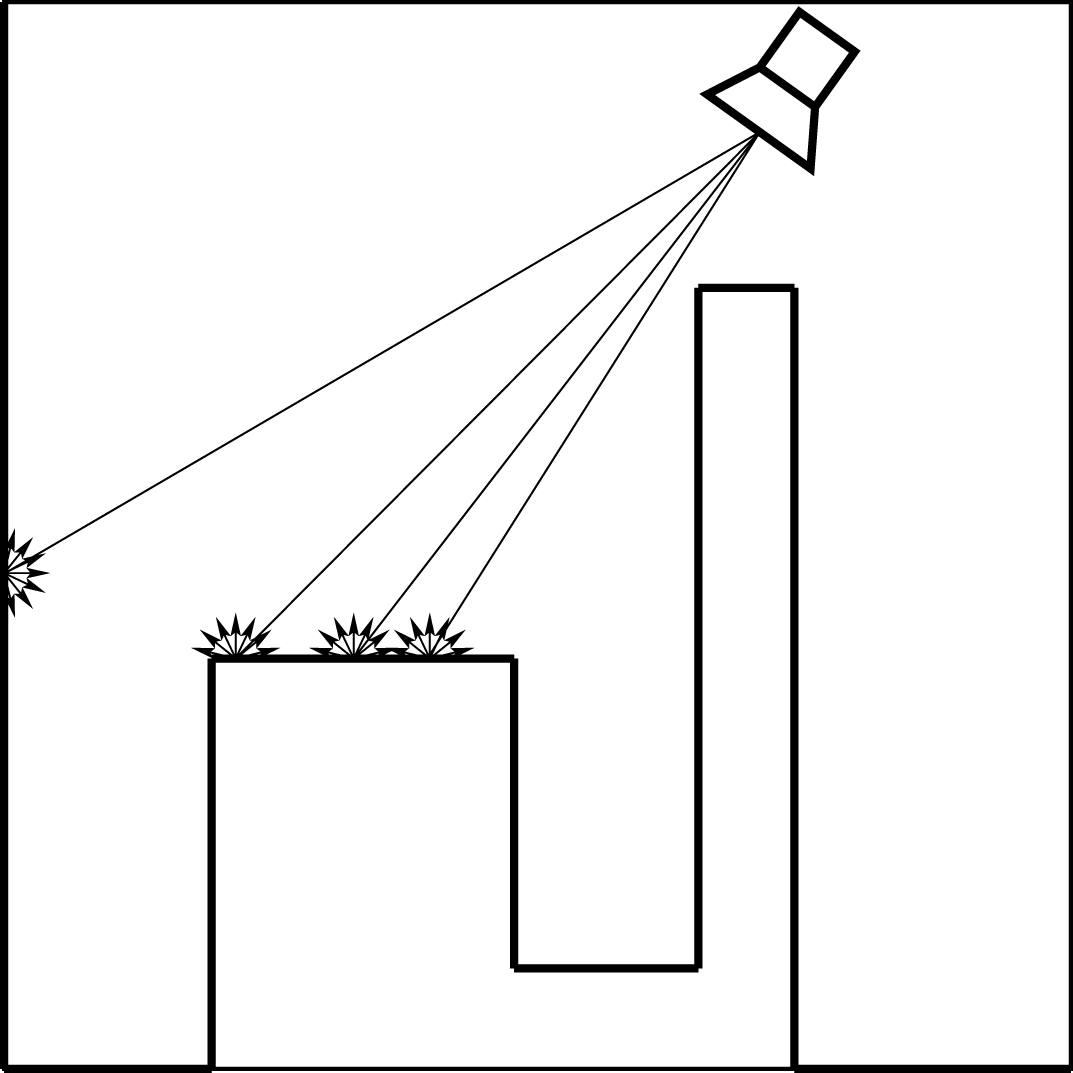
\includegraphics[width=0.9\textwidth]{graphics/lpv/lpv-2-1}
	\caption{Secondary light}
\end{subfigure}
\begin{subfigure}[b]{0.32\textwidth}
	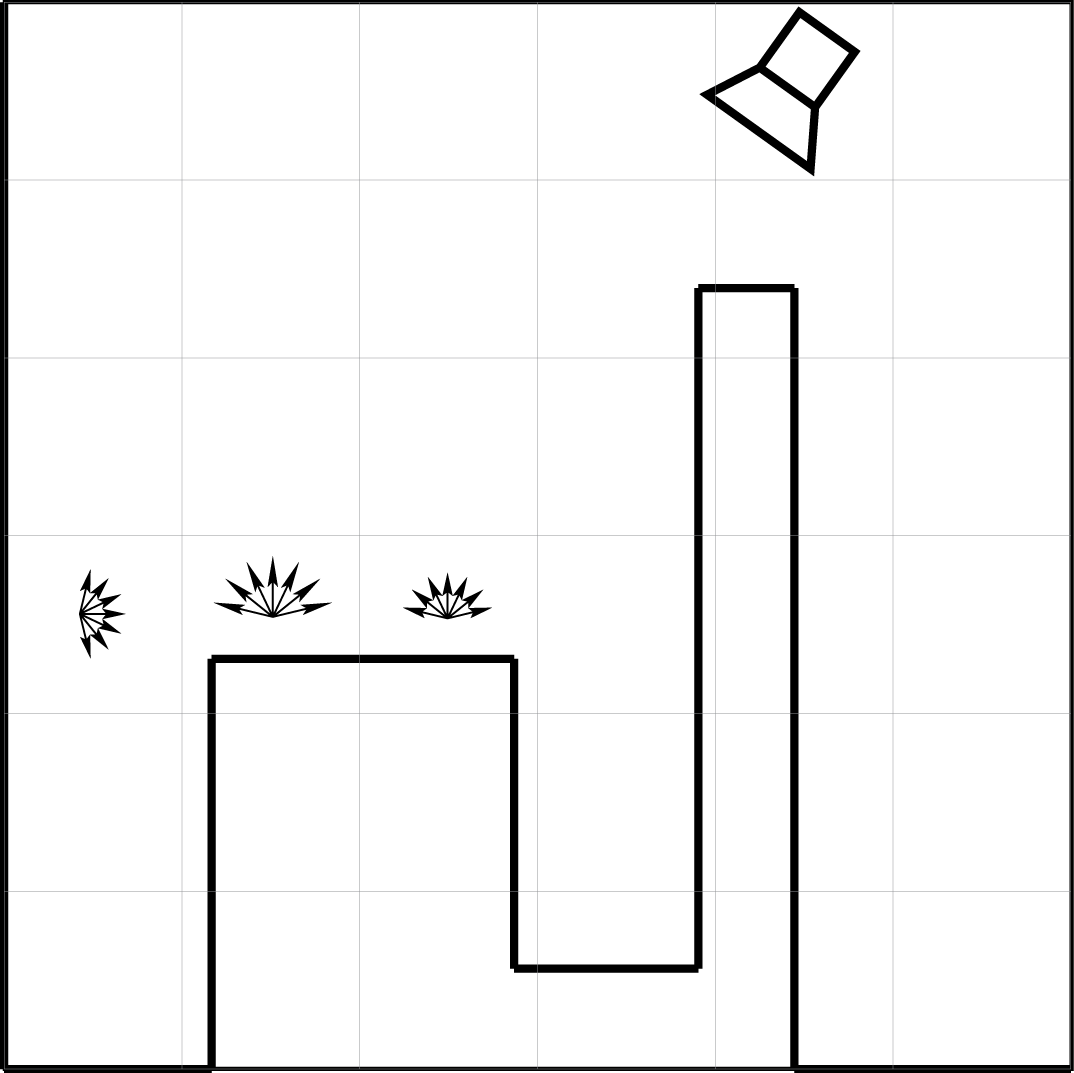
\includegraphics[width=0.9\textwidth]{graphics/lpv/lpv-2-2}
	\caption{Initial distribution}
\end{subfigure}
\begin{subfigure}[b]{0.32\textwidth}
	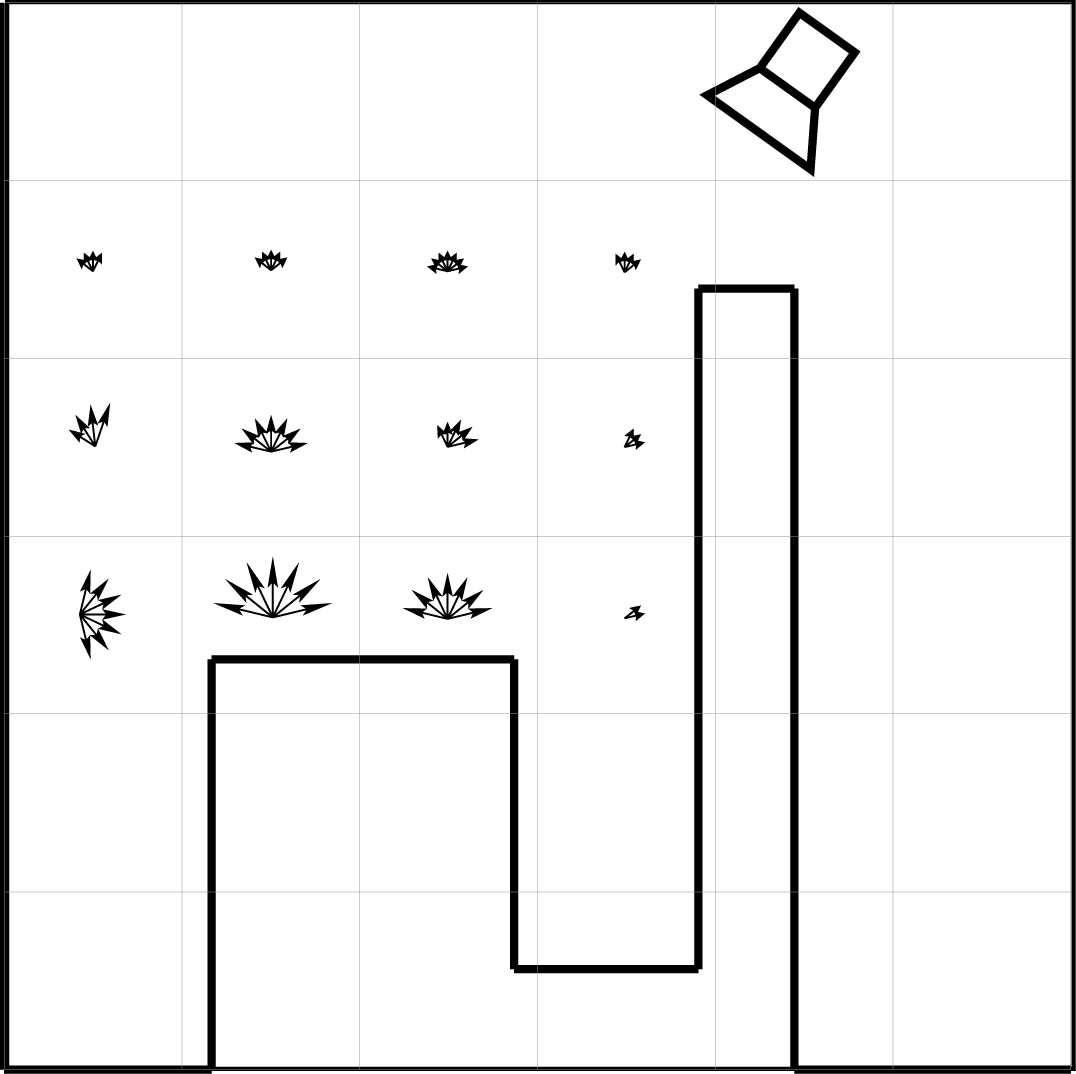
\includegraphics[width=0.9\textwidth]{graphics/lpv/lpv-2-3}
	\caption{Propagation}
\end{subfigure}
\caption{The basic idea of light propagation volumes method.}
\end{figure}

The basic idea is simple. Consider the primary light source emanating light rays. Assuming the whole scene consists of only diffuse surfaces. Each ray excites a secondary emission of bounced radiance along a visible hemisphere of every lit surface element, see figure \ref{f:lpv-basic-idea}(a). Then we introduce a regular 3D grid. Approximate the bounce by binning it into the grid. Accumulate all the bounced results inside of each cell into the cell. Thus we have an initial accumulated indirect radiance distribution, see figure \ref{f:lpv-basic-idea}(b). After we've got the initial reflected light distribution in the grid, we propagate the radiance iteratively around the 3D grid until the light passes the entire grid, see figure \ref{f:lpv-basic-idea}(c).

Computing the indirect lighting with this technique consists of four subsequent steps (as in figure \ref{f:lpv-process}):

\begin{marginfigure}
\begin{center}
	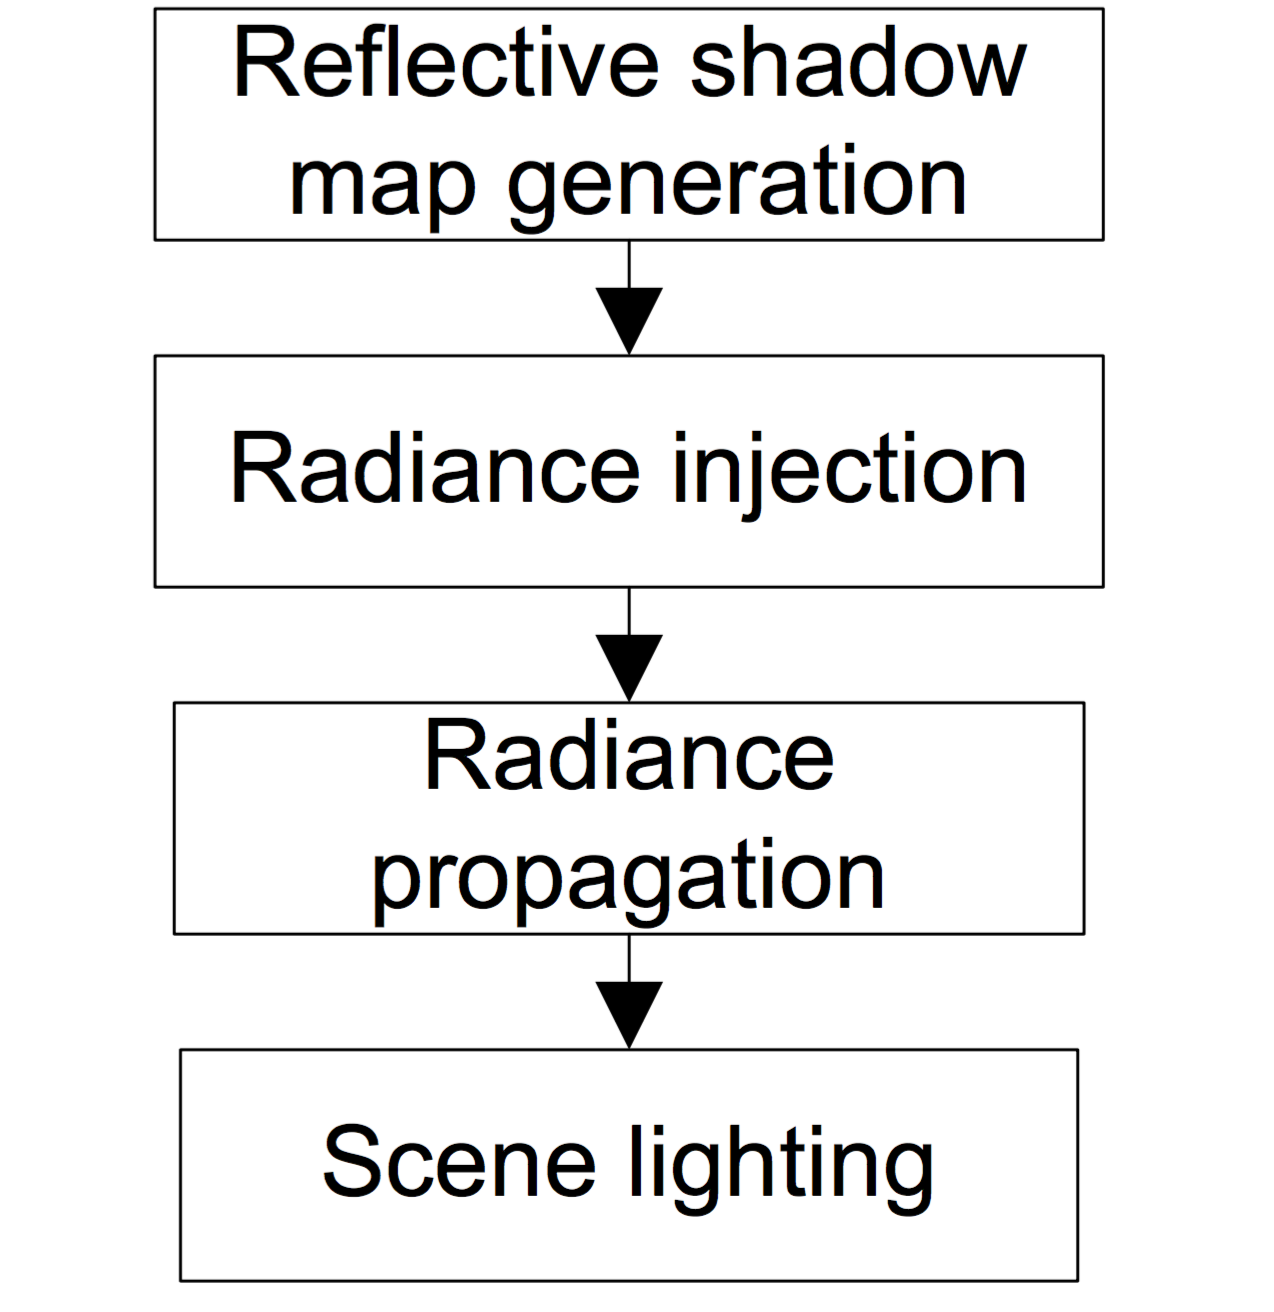
\includegraphics[width=0.8\textwidth]{graphics/lpv/lpv-1}
\end{center}
	\caption{Algorithm overview.}
	\label{f:lpv-process}
\end{marginfigure}

\begin{itemize}
	\item \textbf{Generation of radiance point set scene representation} This stage consist of generation of set of secondary light sources by rendering the scene into reflective shadow map.
	\item \textbf{Injection of point cloud of virtual light sources into radiance volume} Given a point cloud set of virtual light sources from previous stage, inject it into the radiance field which is represented by a volume texture of spherical harmonics coefficients.
	\item \textbf{Volumetric radiance propagation} Within the initial radiance distribution, propagate radiance by iteratively solving differential scheme inside the volumetric grid. Store the results in the radiance volume.
	\item \textbf{Scene lighting with final light propagation volume} Apply resulting radiance volume to the scene lighting. 
\end{itemize}




\subsection{LPV Initialization and Injection}
Light propagation volume is used to compute the low-frequency lighting in a scene only, i.e. mainly the indirect light. Strong direct lighting and shadowing from point or directional light sources is computed using traditional techniques such as shadow mapping.

The initionalization is based on the idea that one can convert the low-frequency lighting into a set of virtual point lights (VPLs), in the spirit of instant radiosity\cite{a:InstantRadiosity}, see chapter \ref{chp:instant-radiosity}. However, it uses a significantly larger number of VPLs than typical instant radiosity methods, since it does not compute their contribution individually, but only uses them to initialize the LPV.

\begin{figure}\label{f:lpv-rsm}
\begin{subfigure}[b]{0.32\textwidth}
	
\includegraphics{graphics/lpv/lpv-3-1}
	\caption{Depth}
\end{subfigure}
\begin{subfigure}[b]{0.32\textwidth}
	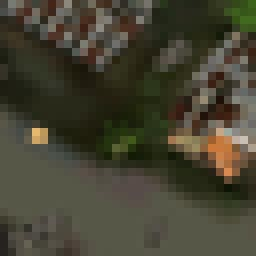
\includegraphics{graphics/lpv/lpv-3-2}
	\caption{Flux}
\end{subfigure}
\begin{subfigure}[b]{0.32\textwidth}
	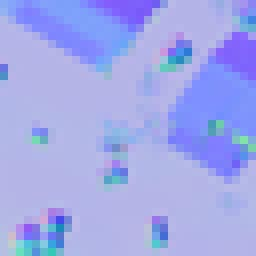
\includegraphics{graphics/lpv/lpv-3-3}
	\caption{Normal}
\end{subfigure}
\caption{Reflective Shadow Maps are an extension of shadow maps and store not only depth, but also normal and reflected flux of the surface seen from the light source.}
\end{figure}

It uses Reflective Shadow Maps (RSM), see figure \ref{f:lpv-rsm}, to generate many secondary light sources. This is a very fast method to sample lit surfaces of the scene on GPU. All pixels of such a shadow map can be seen as indirect light sources that generate the one-bounce indirect illumination in a scene. Each texel of a RSM can be interpreted as a small area light source with a spectral and directional intensity distribution, $I_p(\omega)$, determined by the orientation $\mathbf{n}_p$ of the texel and its reflected flux $\Phi_p$:

\begin{equation*}
	I_p(\omega)=\Phi_p\langle\mathbf{n}_p|\omega\rangle_+
\end{equation*}

where $\langle .|. \rangle_+$ denotes the dot product with negative values clamped to zero. The next step is to transform all VPLs into the SH representation and store their contributions in the LPV cells\sidenote{We can easily determine the cell in which the VPL resides. However, if the VPL points away from that cell's center, we do not want to add its contribution to this cell, but rather to the next cell in order to avoid self lighting and shadowing. For this, we virtually move each VPL by half the cell spacing in the direction of its normal, before determining the cell.}. In that cell, we only take the orientation of the VPL into consideration, i.e. we ignore its exact positioning inside that cell.

It uses SH to represent the directional distribution of intensity. It can easily derive analytical expressions for the SH coefficients of a clamped cosine-lobe centered around a given direction vector, the VPL normal $\mathbf{n}_p$ is this case. A clamped cosine oriented along the z-axis can be expressed in zonal harmonics\cite{a:Ontherelationshipbetweenradianceandirradiance:determiningtheillumina-tionfromimagesofaconvexlambertianobject.}, and rotated to the direction $\mathbf{n}_p$, see algorithm \ref{al:spherical-harmonics-projections}. We can scale these coefficients by the flux to obtain the SH coefficients for a VPL.

Note that the flux of a VPL already accounts for the area of the pixel from which a VPL has been created. Thus there is no further scaling required, and we can accumulated the intensities, i.e. the coefficients of the SH approximation, in the grid cells. In fact, it uses 3 coefficient vectors to represent RGB data.

\begin{algorithm}\label{al:spherical-harmonics-projections}
\begin{lstlisting}[language=C++]
half4 SHRotate(const in half3 vcDir, const in half2 vZHCoeffs)
{
	// compute sine and cosine of thetta angle
	// beware of singularity when both x and y are 0 (no need to rotate at all) 
	half2 theta12_cs = normalize(vcDir.xy);
 	
	// compute sine and cosine of phi angle
	half2 phi12_cs;
	phi12_cs.x = sqrt(1.h - vcDir.z * vcDir.z); 
	phi12_cs.y = vcDir.z;
	
	half4 vResult;
	// The first band is rotation-independent
	vResult.x = vZHCoeffs.x;
	// rotating the second band of SH
	vResult.y = vZHCoeffs.y * phi12_cs.x * theta12_cs.y; 
	vResult.z = -vZHCoeffs.y * phi12_cs.y;
	vResult.w = vZHCoeffs.y * phi12_cs.x * theta12_cs.x;
	return vResult;
}                                                                              
\end{lstlisting}	
\caption{Arbitrary Rotation of function with circularly symmetry around $z$. This method that takes a direction and zonal harmonics coefficients as an input and returns SH coefficients of this function rotated towards given direction.}
\end{algorithm}

Every VPL is treated in this way and then "inject" into the LPV. The Reflective Shadow Map is an input data for this stage. We use point rendering to position each VPL of the RSM into the 3D grid. Generate clamped cosine lobe of radiant intensity distribution in SH out of orientation and colored intensity of each texel of RSM. We use additive blending to efficiently accumulate contribution of all VLPs from RSM in parallel on GPU. Thus we've got a 3D grid initialized by the initial distribution of reflected light in the end of this process.

\begin{figure}
\begin{center}
	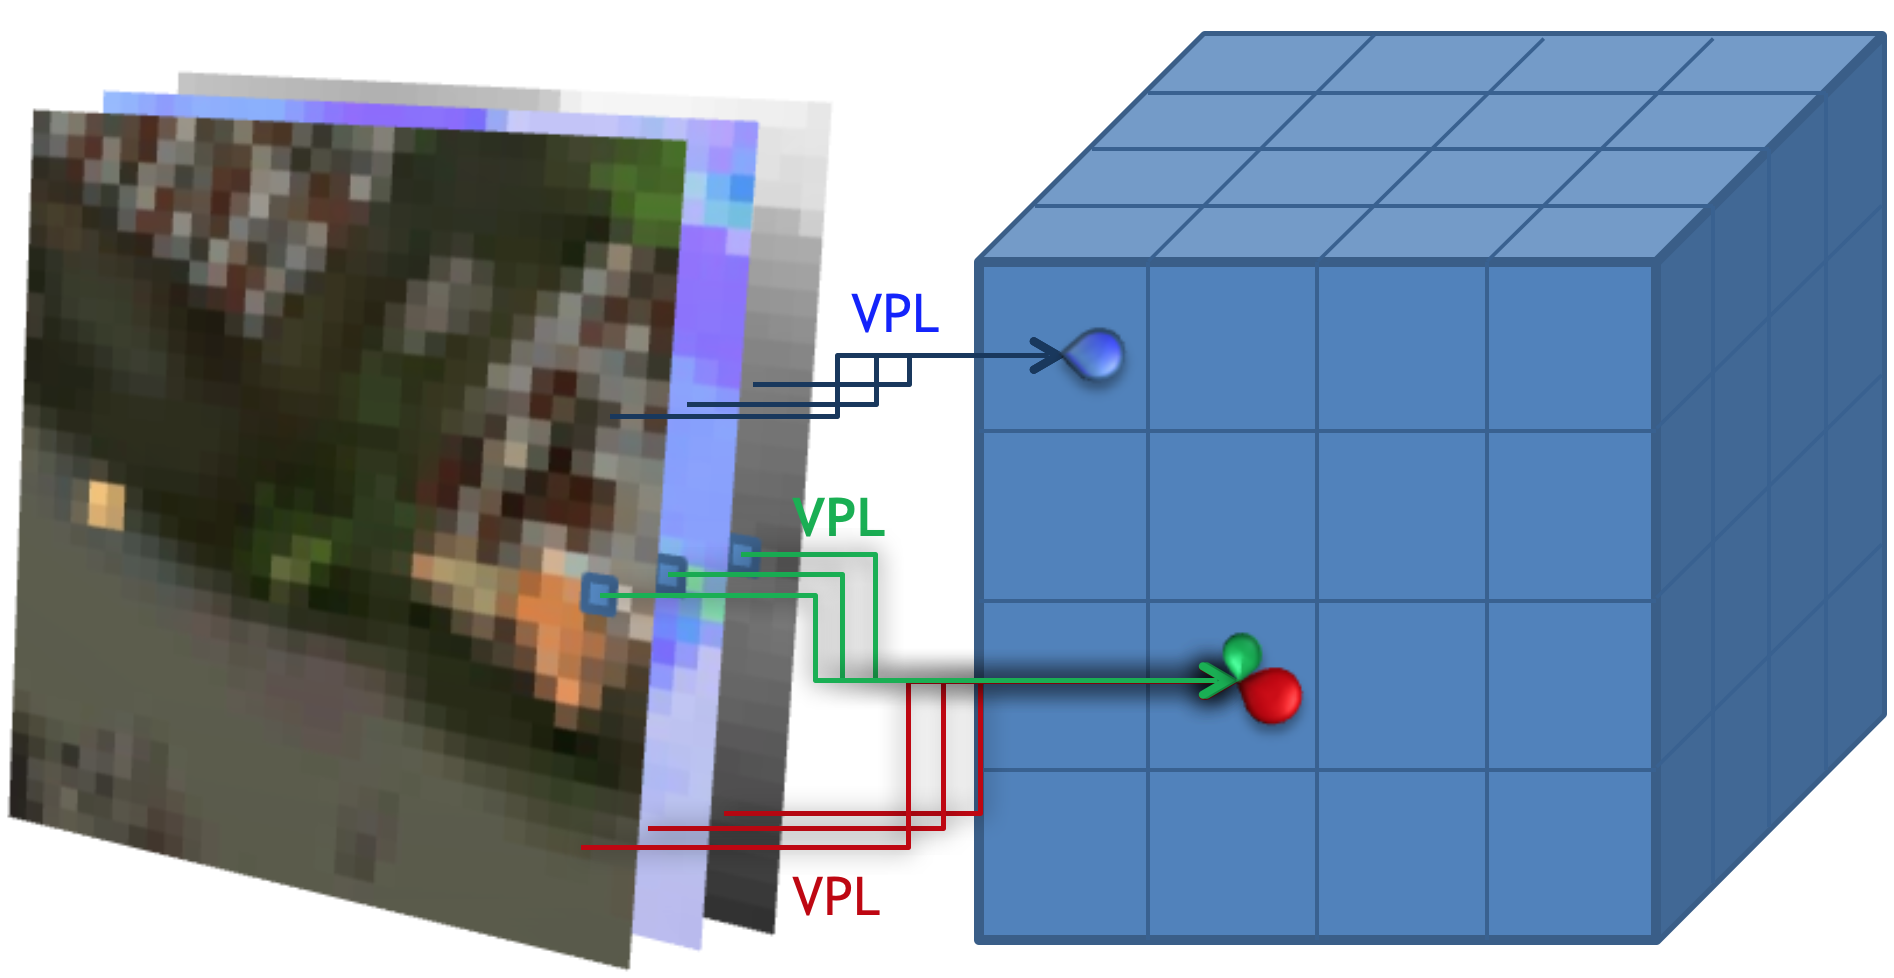
\includegraphics[width=0.6\textwidth]{graphics/lpv/lpv-4}
\end{center}
\caption{The Reflective Shadow Map is an input data for injection. Note in the cell, we only take the orientation of the VPL into consideration, i.e. we ignore its exact positioning inside that cell.}
\end{figure}




\subsubsection{Low-frequency Direct Light}
The second kind of VPL accounts for low-frequency direct lighting from area lights, environment maps and larger groups of point lights, such as those stemming from particle systems. Again, we create a dense sampling, i.e. several hundreds to thousands of VPLs for these light sources, and inject them into the LPV in exactly the same way as those created from RSMs.




\subsection{Scene Geometry Injection}
In LPV, there are two grids, one storing the intensity that is initialized from the surfaces causing indirect lighting or low-frequency direct lighting, as we've seen in the last section; and a second grid that stores a volumetric approximation of the scene geometry and is used for fuzzy blocking which is an approximated occlusion distribution between any two adjacent cells of the LPV. Both grids store a spherical function represented as low-frequency SH approximation.

It aims at fully dynamic scenes without precomputation and consequently this information has to be created on the fly as well. To this end, we re-use the sampling of the scene's surfaces that is stored in the depth and normal buffers of the camera view (using a deferred renderer) and in the RSMs\sidenote{Note that we typically created RSMs for numerous light sources and thus have a dense sampling of a large portion of scene's surfaces.}.

Each sample represents a small surface element (\textit{surfel}) with a given location, orientation, and size. We model the occlusion in spirit of \cite{a:AUnifiedHierarchicalAlgorithmforGlobalIlluminationwithScatteringVolumesandObjectClusters}, and assume that we can use the accumulated blocking potential of surfels in a grid cell as a probability for blocking light from a certain direction going through that cell. By this, we can render soft shadows, but surfaces smaller than the grid size, e.g. foliage, do not produce resolved shadows, in which we can use ambient occlusion.

This grid is shifted by half-cell in all direction so the cell centers of this grid lay exactly on the cell corners of the LPV. We approximate this occlusion distribution function by SH basis as well, see figure \ref{f:lpv-occlusion-grid}. We use rasterization to obtain the occlusion surface elements from the scene. We reuse multiple depth + normal buffers: from light position and from viewer position. The occlusion accumulation process is very similar to the light injection process mentioned before. 

\begin{marginfigure}
	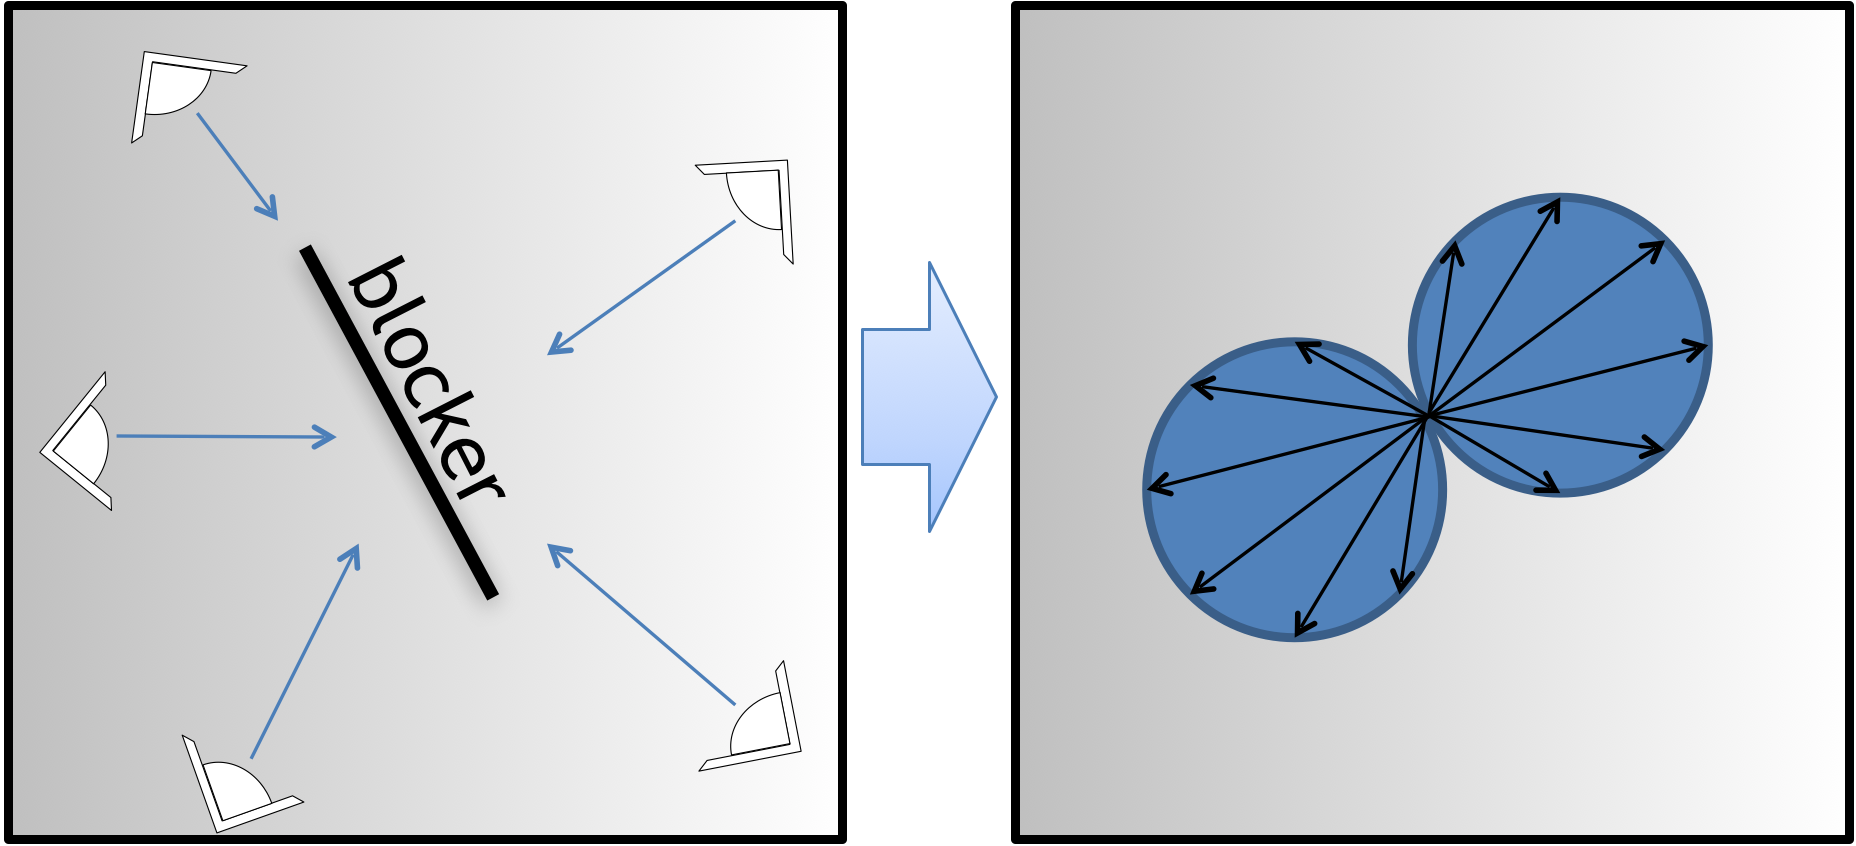
\includegraphics{graphics/lpv/lpv-5-1}
	\caption{Since occlusion area is view dependent we could represent it as a function of the view direction, as shown on the left picture. This function represents a cosine lobe for a simple occlusion element (right figure).}
	\label{f:lpv-occlusion-grid}
\end{marginfigure}

The amount of blocking by one of these surfels depends on its size, and on the cosine of the angle between its normal and the light direction. The blocking probability of a single surfel with area $A_s$, and normal $\mathbf{n}_s$ in a cell of grid size $s$ is thus:

\begin{equation*}
	B(\omega)=A_s s^{-2}\langle \mathbf{n}_s|\omega\rangle _+
\end{equation*} 

Since the cells of the occlusion grid are on the corners of the LPV, we need to retrieve the occlusion distribution in between of the source occlusion cells for propagation occlusion. We use bilinear interpolation of SH coefficient for that, see figure \ref{f:lpv-interpolation}.

\begin{marginfigure}
	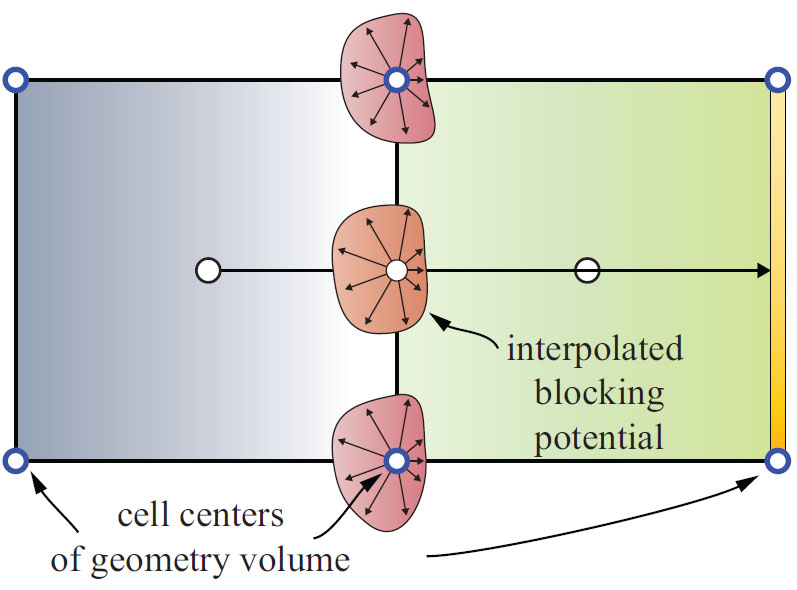
\includegraphics{graphics/lpv/lpv-5-2}
	\caption{We account for fuzzy occlusion by storing a volumetric representation of the scene in a second grid. And retrieve the occlusion by bilinear interpolation.}
	\label{f:lpv-interpolation}
\end{marginfigure}




\subsection{Propagation Scheme}
After we've got an approximation of outgoing indirect lighting in each cell of our 3D grid, we can apply an iterative process of energy propagation across the grid.



\subsubsection{Intensity Propagation}
The input for the first iteration step is the initial LPV from the injection stage, subsequent iterations take the LPV from the previous iteration as input. Each cell stores the intensity as a SH-vector and the light is then propagated to its 6 neighbors alonge the axial directions, see the left of figure \ref{f:lpv-propagation}.

\begin{figure}\label{f:lpv-propagation}
	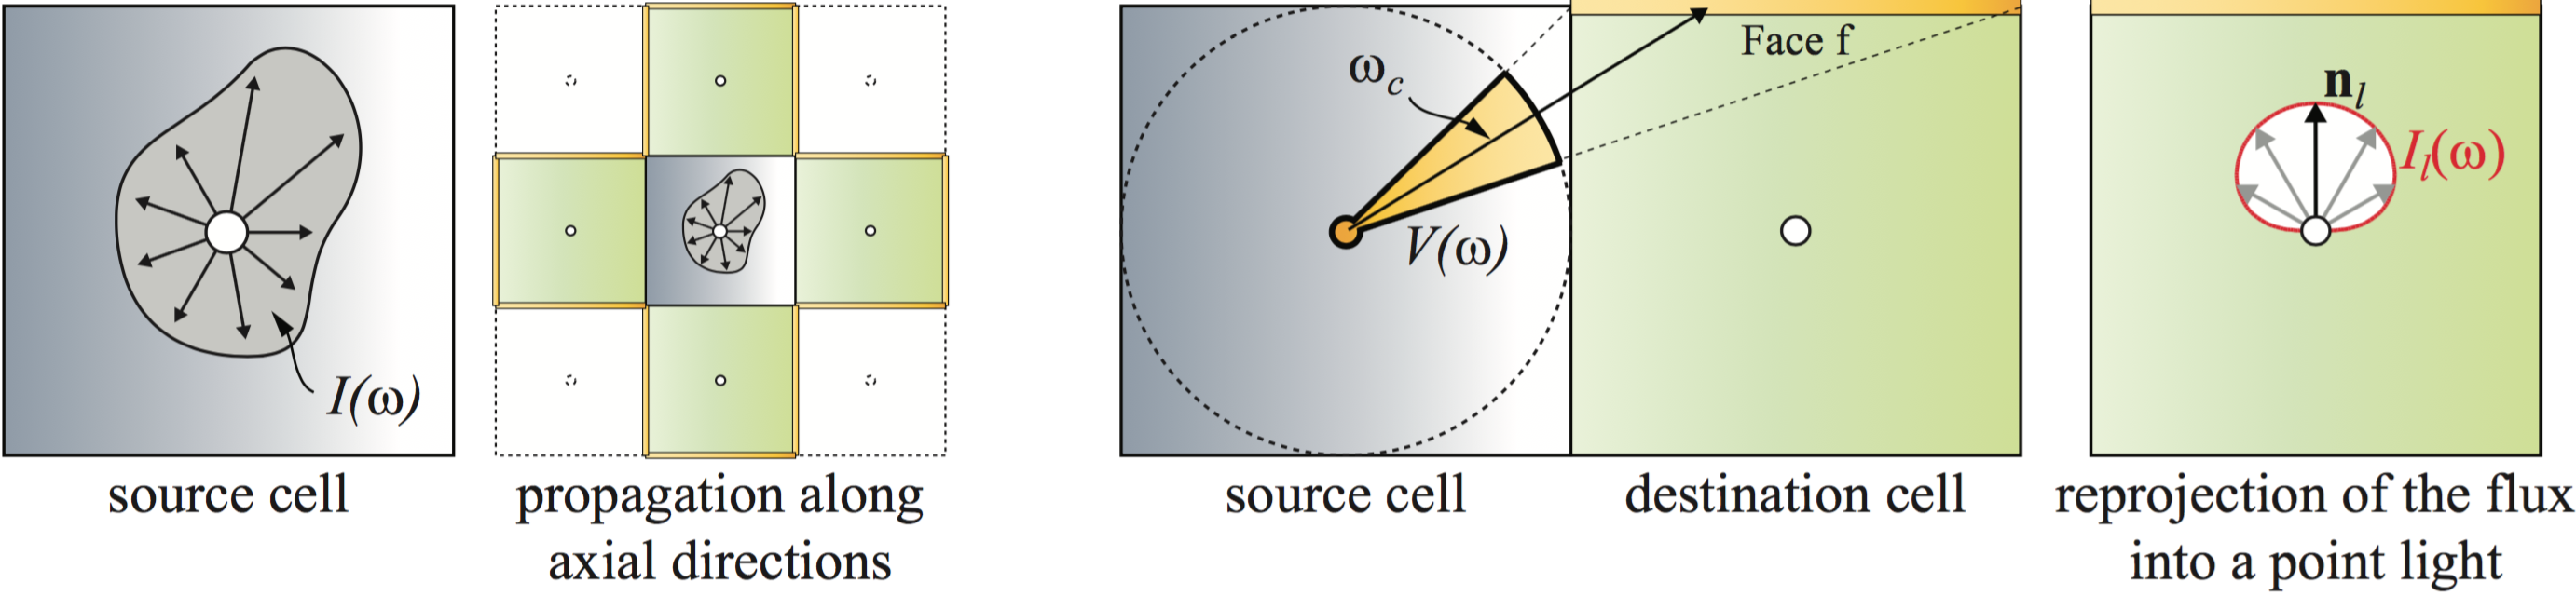
\includegraphics{graphics/lpv/lpv-6-2}
	\caption{Left: Each cell of the LPV stores the directional intensity used to compute the light that is propagated from a source cell to its 6 (4 in 2D) neighbors. Center: We compute the flux onto the faces of the destination cell to preserve directional information.}
\end{figure}

Denote the SH-approximation of the intensity of the source cell as:

\begin{eqnarray*}
	I(\omega)\approx\sum_{l,m}c_{l,m}y_{l,m}(\omega)
\end{eqnarray*}

Next we compute the flux onto each of the faces of the adjacent destination cell. For this we define the visibility function, $V(\omega)$, of a face $f$ with respect to the source cell's center. $V(\omega)=1$ if a ray starting at the source cell center in direction $\omega$ intersects the face, otherwise $V(\omega)=0$. The right of figure \ref{f:lpv-propagation} shows $V(\omega)$ for the top face of the destination cell. The total flux reaching the face can be computed by integrating over directions using $V(\omega)$ as:

\begin{equation*}
	\Phi_f=\int_\Omega I(\omega)V(\omega)d\omega
\end{equation*}

The faces' visibility functions can be projected into SH yielding a coefficients vector $v_{l,m}$ with $V(\omega)\approx\sum_{l,m}v_{l,m}y_{l,m}(\omega)$. The integral over intensity times visibility can then be easily computed using the dot product of the SH-vectors $c_{l,m}$ and $v_{l,m}$.

These "transfer vectors" $v_{l,m}$ can be precomputed once and stored for the propagation scheme. The problem, however, is that the integral value can be very inaccurate for low-order SH approximations, and thus they propose using a different strategy for this case. Instead of a transfer vector we compute the solid angle $\triangle\omega_f=\int_\Omega V(\omega)d\omega$ of each face in the destination cell, and determine the central direction $\omega_c$ of the visibility cone. The flux reaching the face is then computed as $\triangle\omega_f/(4\pi)\cdot I(\omega_c)$. Effectively this means that we take the intensity in direction $\omega_c$ as average intensity over the solid angle.




\subsubsection{Reprojection}
Using this propagation we obtain the incident flux for each face of a destination cell and then transform it into outgoing intensity for the subsequent propagation again. It consists of the following steps:

\begin{itemize}
	\item Firstly we create a point light in the center of the destination cell. This light is oriented towards the face and has an intensity which corresponds exactly to the amount of flux produced by the face. That is, the flux on the face, $\Phi_f$, is equal to the total emitted flux of the point light (see the right of figure \ref{f:lpv-propagation}):

		\begin{equation*}
			\Phi_f=\int_\Omega\Phi_l\langle\mathbf{n}_l,\omega\rangle_+d\omega
		\end{equation*}
		
	\item Generate clamped cosine lobe in SH basis similar to injection stage.
	\item Accumulate the resulting contribution of the face into the SH coefficients of the destination cell for the next iteration.
\end{itemize}

The propagation is computed for each source cell and each of its adjacent cell's face (shown yellow in figure \ref{f:lpv-propagation}). Note that this process conserves energy that is expected from light propagation in vacuum. However, the propagation together with the reprojection introduces spatial and directional discretization. Note that this is common to all lattice-based methods.



\subsubsection{Blocking}
We also need to integrate the blocking of light due to scene geometry into the propagation step. In the geometry injection stage we computed the GV from the surfaces in the scene that stores anisotropic occlusion probabilities for exactly this purpose. The GV is displaced by half the grid size with respect to the LPV. By this, a cell center of the GV resides on a corner of an LPV cell. Whenever we propagate from a source to a destination cell, we bi-linearly interpolate the GV's SH-coefficients at the center of the face through which we propagate, and evaluate the occlusion for the propagation direction to attenuate the intensity. Note that we do not consider this occlusion in the very first propagation step after injection in order to prevent self-shadowing.





\subsection{Rendering}
During the final rendering of the scene, we illuminate it by looking up the grid texture with trilinear 3D interpolation of SH coefficients. Then evaluate the irradiance by convolving the obtained radiant distribution with the cosine lobe of the surface's normal. This can be done both in forward rendering and in deferred rendering. Also it works well with alpha-transparent objects.

To avoid unwanted light bleeding through thin objects, we apply a dampening factor in a following way:

\begin{itemize}
	\item Firstly we do another look-up towards the direction of the surface's normal and compute a directional derivative by a finite difference.
	\item Then we dampen the obtained irradiance based on the deviation of the derivative from the direction of intensity distribution itself.
\end{itemize}




\section{Go Further}
In this section we describe further rendering techniques using the LPV, followed by a discussion of benefits and limitations.

\subsection{Multiple Indirect Bounces}
Now we extend the technique to the multiple bounces using LPVs. The idea is to use information from the occlusion grid to compute multiple indirect reflections. When propagating from a source to a destination cell, we perform an additional lookup into the GV with an offset of once cell into propagation direction.



So during each propagation iteration we reflect light by using the information from the occlusion distribution at the receiving face (as shown in figure \ref{f:lpv-multiple-indirect-bounces}). We put the reflected amount of light into the source cell, which means that we introduce a safety-distance for reflected light to avoid a self-illumination.



The result of multiple bounces is depicted on the bottom image. Notice double-bouncing of indirect light from the white box.

\begin{figure}\label{f:lpv-multiple-indirect-bounces}
	\begin{center}
		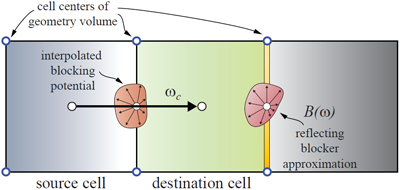
\includegraphics[width=0.7\textwidth]{graphics/lpv/lpv-7}
	\end{center}
	\caption{We use the GV to approximate more bounces of indirect illumination.}
\end{figure}


\subsection{Glossy Reflections}
\subsection{Participating Media}


The virtual point injection is traditionally done via reflective shadow maps that render the scene from the location of each light source and store information such as depth, world space coordinates, normal and flux. This information is then aggregated into two distinct volume data structures, i.e. two three-dimensional regular grids. The first volume stores a set of spherical harmonics coefficients for each cell representing a virtual point light. The second volume is offset by half a cell in each direction and stores a set of spherical harmonics coefficients approximating the occlusion between the cells in the first grid. The spherical harmonics coefficients in both volumes are then iteratively combined to propagate indirect light within the first volume. Finally, applying lighting in the fragment shader simply involves looking up the interpolated value within the light propagation volume which is stored in a volume texture on the GPU. Also, in practice, light propagation volumes employ cascades of regular grids to scale to large environments where the cascades move with the camera location and snap to a world grid to avoid flickering.

Light propagation volumes allow lights, materials and objects to be fully dynamic at runtime. They work well with complex geometry and are relatively stable and flicker-free. At basic quality levels they can even scale down to mobile platforms. In addition, light propagation volumes support multiple bounces, glossy reflections and participating media; however, these extensions are usually considered too expensive in practical applications and the computational resources are rather used to improve the base lighting quality.

Light propagation volumes have a number of issues that limits their application, the biggest being their low spatial resolution due to memory constraints even when employing cascades. Due to this, light and shadow leaking are a common occurrence and the lighting result is fairly ambient with low contrast. In combination with the fact that their runtime performance scales with the number of light sources, light propagation volumes are mostly used for outdoor scenes with only a single directional light source.

Irradiance volumes (like Tatarchuk's presentation "Irradiance Volumes For Games"), is merely a light probe's technique like the post on codeflow.org previously linked.

Crytek mention irradiance is used in conjunction with LPV. Don't confuse the both methods because they are radically different. In their first Siggraph presentation Crytek mention that they are making the two work together because it is a bad idea to inject sky radiance into the LPV. First, because you would need 55 steps of propagation to make the radiance flows all the way down, second because it will disrupt the flux of other lights because of the poor 2 bands SH, and because it will interfere with itself since sky radiance is hemispherical and has to be injected from 5 faces in the LPV, thridly because a volume full of flux makes the limits very noticeable, lastly because this technique is full of leaks, it is better to keep the flux to a minimum.

So they are using classic dome irradiance for contribution of the sky. They don't say how they solve occlusion from the sky's radiance, and I think they do not. That is why it is nowhere mentioned in their second paper.

%
\section{Cascaded Light Propagation Volumes}
\subsection{Nested Grid Propagation}
\subsection{Qualitative Evaluation of the Propagation}
\section{High Order LPV}
%





























